\section{Smart Data Pricing}\label{SDP}

%The demand for data is growing rapidly in both wired and wireless networks. This growth is primarily driven my the rise of mobile video, bandwidth-hungry apps, bulk transfer to the cloud, and user-friendly interfaces of smart devices. The Cisco Visual Networking Index predicts that data from mobile devices will grow to a volume of 10.8 exabytes per month in 2016, while wired network traffic will increase at a compound annual growth rate of 28\% per year \cite{CiscoVNI}. 

%The predicted doubling of demand for mobile data every year also means that technical solutions and spectrum reallocation are going to be insufficient to meet the growing needs of the users. ISPs' (Internet service providers) are therefore turning to new pricing plans in an effort to manage their demand for data and match their prices to cost \cite{comm-mag}. Such policies include charging based on usage volume, throttling users' bandwidth, and imposing caps on monthly usage.  Figure \ref{fig:timeline} provides an overview of the rapidly evolving pricing and demand control practices of the major U.S. ISPs since 2008. In fact, over the past few years, ISPs around the world have started to offer innovative pricing plans, including usage-based and app-based pricing to tackle the problem of network congestion \cite{computing-survey}. 

 \begin{figure}
\centering
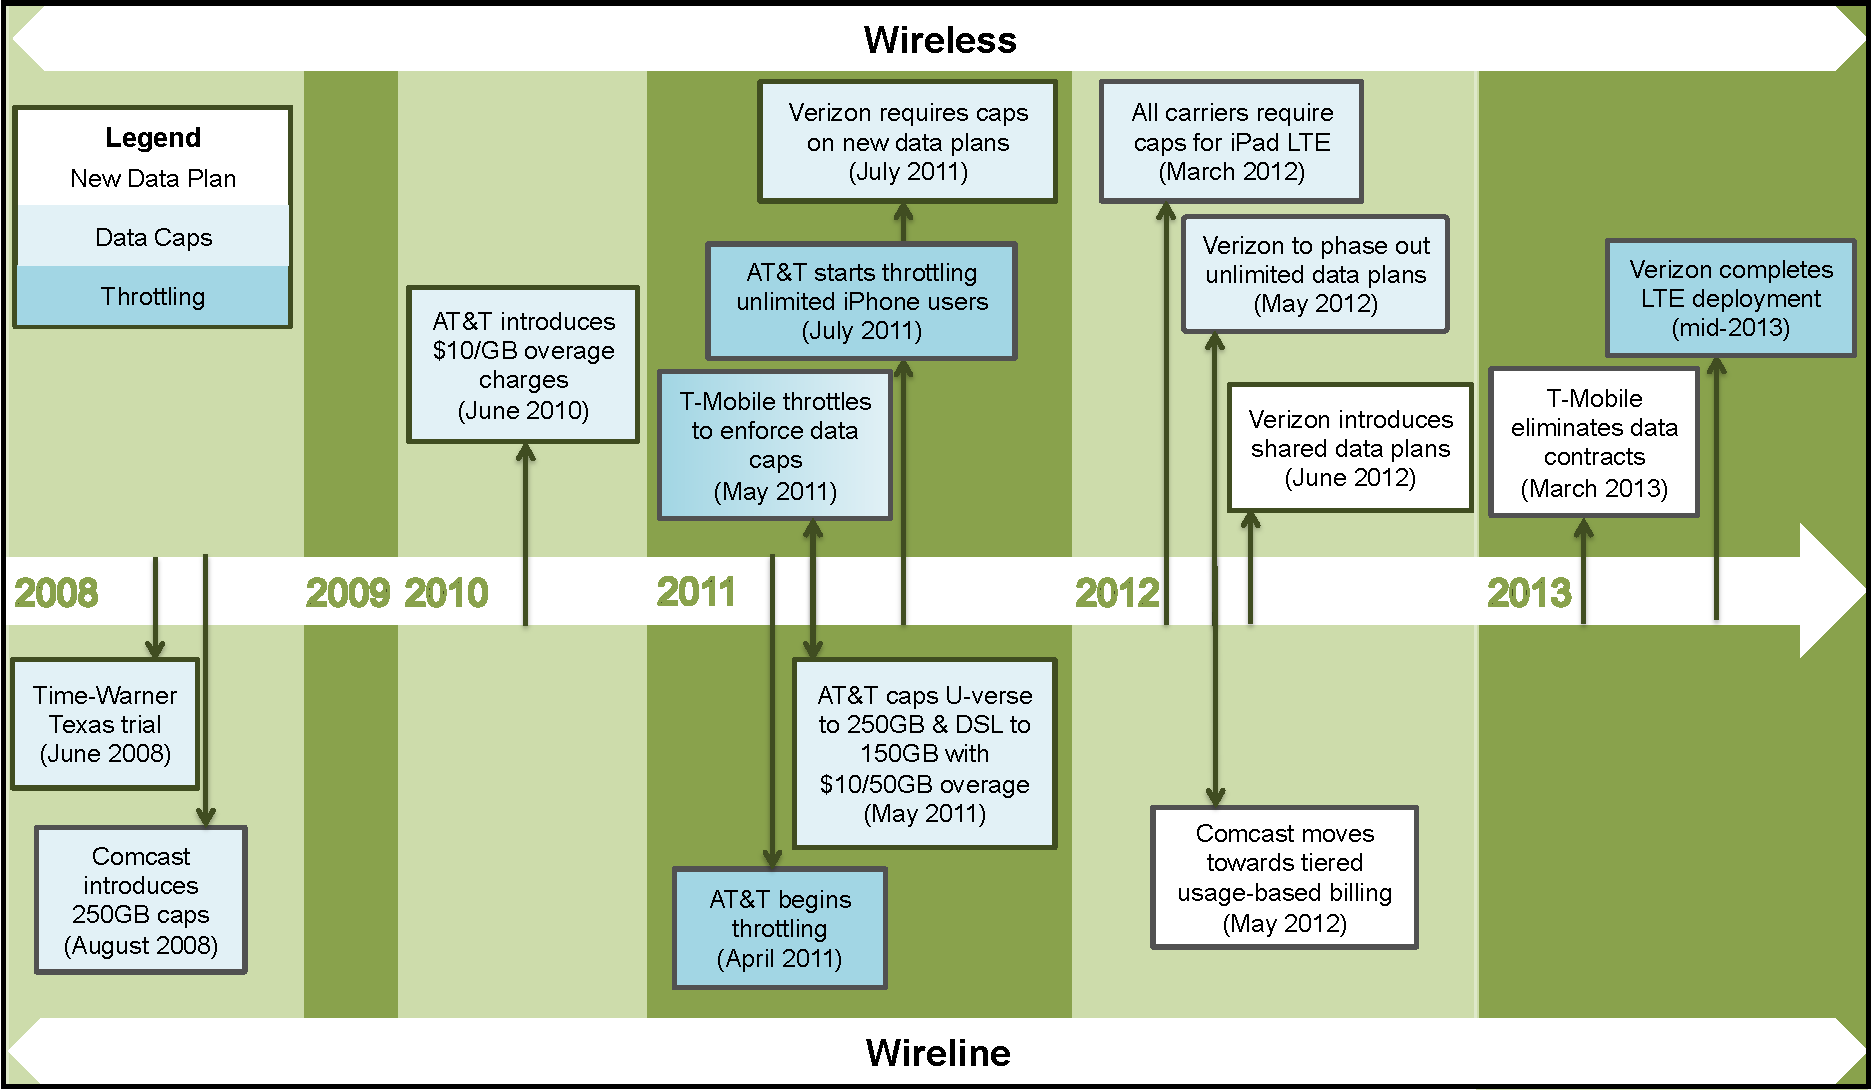
\includegraphics[width = 0.85\textwidth]{Figures/Timeline.pdf}
\vspace{-0.1in}
\caption{Broadband pricing plans offered by major U.S. ISPs, 2008 - 2013.}
\label{fig:timeline}
\vspace{-0.05in}
\end{figure}

Broadband access pricing and demand control practices have rapidly evolved among U.S. ISPs since 2008, as seen in Figure \ref{fig:timeline}. Over the past few years, ISPs around the world have started to offer innovative pricing plans, including usage-based and app-based pricing to tackle the problem of network congestion \cite{computing-survey}. Smart Data Pricing (SDP) \cite{SDP2013} is an umbrella term for a suite of pricing and policy practices that have    
been proposed in the past or are being explored as access pricing options by operators instead of the traditional flat-rate model. Such SDP models can include any or of the following mechanisms or a combination, which will be discussed later in the chapter: (a) Usage-based pricing/metering/throttling/capping, (b) Time/location/congestion-dependent pricing, (c) App based pricing/sponsored access, (d) Paris metro pricing, (e) Quota-aware content distribution, (f) Reverse billing or Sponsored Content. SDP does not even need to be an explicit pricing mechanism; it can be another form of innovative congestion management like WiFi offloading or ``fair-throttling''\footnote{Fair throttling involves accounting for user's usage history of contributing to congestion in determining what share of available bandwidth the user should receive in a congested time.}.

The basic ideas of congestion pricing have received much attention as a research topic both in computer networks and information systems literature, and are once again getting a fresh look from academics in recent years. Given the change in the economic and regulatory environment of Internet pricing, it is likely that some of the ideas will be realized in future data plans. However, research in the design of such smart data pricing plans should account for some new factors: (i) the growth in traffic with high time-elasticity of demand (e.g., downloads, P2P, cloud backup, M2M) and the ability to schedule such traffic to a less congested time without user-intervention, (ii) revisiting the issue of dividing the elements of a congestion control-feedback loop between the network backend and the smart end-user devices, (iii) development of new system architectures to deploy these pricing ideas and demonstration of their potential benefits through field trials. In other words, it requires understanding both the \emph{economic theory} of pricing models as well as the \emph{systems engineering} and \emph{human-computer interaction} aspects of realizing such data plans. These require a multi-disciplinary approach in SDP research that bridges theory, systems, and user trials by drawing on economic theory, network engineering and user behavioral studies in a collaborative environment, as shown in Figure \ref{fig:theme}.

 \begin{figure}
\centering
\includegraphics[width = 0.5\textwidth]{Figures/Sdp-theme.pdf}
\vspace{-0.1in}
\caption{Smart Data Pricing research components}
\label{fig:theme}
\vspace{-0.05in}
\end{figure}

% Unfortunately, most academic materials presently available online tend to only provide just enough background on congestion pricing models from a theoretical perspective, rather than taking a more holistic approach.  In particular, most of the materials on economic aspects of the Internet available to students and faculties are either technical papers from conferences such as ACM SIGCOMM, NetEcon, CoNEXT, INFOCOM or edited books of workshop proceedings \cite{MIT}. It is arguably fair to say that most networking textbooks do not cover this important topic in enough depth, and this lack of background materials at the graduate level is indeed a serious issue that the community is now reckoning with. There is a growing realization in the network research community about the need to include network economics as an integral part of engineering curriculum given the complex interplay between technological and economic factors. To this end, we propose to bridge this gap by contributing a chapter that exclusively focuses on the network economics of smart pricing practices for the Internet. 


%The key elements of this chapter will be: (i) a detailed overview of pricing proposals, (ii) system design considerations in smart pricing, and (iii) human factors and results of pricing trials of SDP plans. % The authors have been deeply involved in studying pricing plans, published survey articles and research papers on SDP, and have conducted real trials of SDP with ISPs in US and India, which will inform the contents presented in this contribution.   Additionally, the authors will seek inputs from their collaborators and peers  with whom they have been working closely for network economics research,  especially Prof. Andrew Odlyzko of the University of Minnesota and Prof. Roch Guerin of the University of Pennsylvania, both of whom were invited keynote speakers at the first SDP workshop hosted by the authors in Princeton University in 2012 \cite{SDPForum}. We would also provide a summary of open questions and challenging directions in network pricing, along with supplementary background materials, that can benefit graduate students in identifying new research directions to pursue.

% In the following sections, we first provide an overview of the driving factors behind network congestion in Section \ref{sec:factors}. This rising demand for bandwidth has led to new threats to the current Internet ecosystem: ISPs are increasingly feeling a capacity crunch on their networks, leading to new pricing plans that have raised concerns among consumers hit with these new forms of pricing. Content providers, whose videos and other content make up the increased traffic volume that consumers are demanding, also have a stake in this evolving ecosystem, as do application developers and government regulators attempting to find a balance between ISP capacity concerns and Internet availability. We discuss these different perspectives in Section \ref{sec:threats}. In Section \ref{sec:econ}, we consider a few examples of SDP to illustrate key economic concepts essential for understanding the SDP literature. Section \ref{sec:congestion} gives an overview of this literature, including some pricing plans from the electricity and transportation industries that can be applied to broadband pricing. We then delve into one such pricing plan, day-ahead time-dependent pricing, in order to illustrate the end-to-end nature of an SDP deployment, which requires developing pricing algorithms, designing an effective interface for communicating those prices to users, and implementing an effective system to communicate between an ISP and its users. Finally, we point to some (of many) research questions for broadband access pricing that have yet to be answered.

